\documentclass[11pt]{article}
\usepackage[T1]{fontenc}
\usepackage{lmodern,amsmath,amssymb,amsthm,mathtools,microtype}
\usepackage[letterpaper,margin=.9in]{geometry}
\usepackage{tikz}
\usepackage{booktabs}
\usepackage{hyperref}
\hypersetup{pdfauthor={Peyton Wang and Daniel Wang},pdftitle={Chamber Pockets and an Infinite Lit Family of 20-Wall Rooms},colorlinks=true,linkcolor=black,citecolor=black,urlcolor=blue}
\setlength{\parindent}{0pt}
\setlength{\parskip}{4pt plus 1pt minus 1pt}
\newtheorem{theorem}{Theorem}
\newtheorem{lemma}{Lemma}
\newtheorem{proposition}{Proposition}
\newtheorem{corollary}{Corollary}
\theoremstyle{definition}
\newtheorem{definition}{Definition}
\theoremstyle{remark}
\newtheorem{remark}{Remark}
\newcommand{\Z}{\mathbb Z}
\newcommand{\R}{\mathbb R}
\newcommand{\interior}{\operatorname{int}}
\def\UrlBreaks{\do\/\do-\do\.\do\_}
\newcommand{\repopath}[1]{\nolinkurl{#1}}
\title{Chamber Pockets and an Infinite Lit Family\\of 20-Wall Rooms}
\author{Peyton Wang\\\small Francis Parker School \and Daniel Wang}
\date{Working draft v0.1 --- 23 November 2026\\\small Not submitted or peer reviewed}
\begin{document}
\maketitle
\begin{abstract}
A rectangular pocket with a solid roof and two solid sides acts on a billiard
ray entering through its mouth as a rotation of an oriented phase circle:
the return position is the entry position shifted by $2hc$ modulo $2w$,
where $w$ and $h$ are the pocket's width and height and $c$ is the ray's
horizontal travel per unit rise. This note uses that return map to light an
infinite family of strictly simple orthogonal lattice rooms with 20 walls.
Three aligned $3\times 3$ chambers are joined by two unit corridors of equal
length; the chamber spacing is $D=3k+4$ and the area is $29+6k$.
For every $k\ge 1$, every pair of distinct interior lattice points is lit.
The decisive pair needs at least two horizontal reversals, and an explicit
excursion into the middle chamber's upper pocket supplies them.
The note also gives an exact matching criterion for pocket excursions,
which extends the theorem to independent corridor lengths;
phase maps for paths that reflect inside unit necks, with a lit
$3\times 4$ middle-chamber family; and a group-ring coefficient $J$ that is
positive exactly when a prescribed sequence of strip transits exists.
The results concern specified room families and lattice endpoints.
They give no general wall-count bound.
\end{abstract}

\section{Introduction}
The rooms studied here are three rectangular chambers joined in a row by two
rectangular necks. Each neck is strictly inset at both ends, so each costs four
reflex corners, and two necks use the eight reflex corners available to a room
with 20 walls. An earlier review identified the aligned family with
three $3\times 3$ chambers and corridor lengths $X=Y=3k+1$
\cite{d152}. A later review found that the unfolding monodromy of this family is
primitive for most $k$, so factor-type certificates of illumination do not exist
there \cite{d199}. A direct path construction is therefore needed.

Theorem~\ref{thm:three} gives that construction. Every pair of distinct interior
lattice points is lit, for every $k\ge 1$. Most pairs are joined by a straight
segment, one bounce, or a seam-matched fold. The exception is a pair at equal
offsets in the two outer chambers. Proposition~\ref{prop:reversal} shows that
no legal path with zero or one horizontal reversal joins it. The path that does
join it climbs into the part of the middle chamber above the corridor band,
crosses $2k+2$ side-wall images, reflects once at the roof, and returns to the
band one unit to the right of where it entered, on the rightward sheet.

Section~\ref{sec:pocket} isolates the mechanism. A pocket's return map is a
phase shift (Lemma~\ref{lem:pocket}), and Proposition~\ref{prop:match} gives an
exact criterion for when the shift connects a prescribed source leg to a
prescribed target leg. The criterion removes every congruence and equality
assumption from Theorem~\ref{thm:three} (Theorem~\ref{thm:unequal}).
Section~\ref{sec:neck} treats paths that reflect inside unit necks, and
Section~\ref{sec:groupring} encodes a prescribed list of strip transits as an
identity coefficient in a finite group ring.

The 22-wall room R22 with one dark pair does not have the three-chamber
decomposition used here, so its dark pair does not conflict with these
theorems \cite{d154,R1}. None of the results bounds the number of walls of a dark
room in general.

Each main result has an independent AI review. The reviews found no error in a
proof step. Their corrections and stated gaps appear in the text at the point
where they apply. Section~\ref{sec:scope} lists what remains open.

\section{Setup and conventions}\label{sec:setup}
\paragraph{Rooms.} A \emph{room} is the closed region bounded by a Jordan
polygonal curve. Throughout, rooms are \emph{strictly simple orthogonal lattice
rooms}: every edge is horizontal or vertical, every vertex has integer
coordinates, and the room has no holes, self-contacts, or interior mirrors.
Every wall is therefore a lattice segment. A room with $W$ walls and $r$ reflex
corners satisfies $W=2r+4$, so $W=20$ allows exactly eight reflex corners.
An \emph{interior lattice mark} is a point of $\interior(P)$ with integer
coordinates.

\paragraph{Lit and dark.} A \emph{legal billiard path} has finitely many
straight legs, reflects specularly at smooth boundary points, and never meets a
vertex. Two distinct interior points are \emph{lit} (they illuminate one
another) if a legal path joins them; otherwise the pair is \emph{dark}.
A \emph{horizontal reversal} is a reflection at a vertical wall, where the
horizontal velocity changes sign.

\paragraph{Unfolding.} Reflect the room across each wall a path meets. The path
develops into a single straight segment, and the reflected copies of the room
it passes through form its unfolding. Conversely, a straight segment in a chain
of reflected copies folds back to a legal path whenever it crosses each
reflecting wall image at a smooth point and each opening in the interior of the
opening. Reflection in a line $y=m$ with $m\in\Z$ maps $y$ to $2m-y$, so a
composition of such reflections has the form $y\mapsto \pm y+2m'$ with
$m'\in\Z$. Lattice points remain lattice points in every copy.

\paragraph{Strips and phases.} Unfold the two walls $x=0$ and $x=w$ of a strip
$(0,w)\times I$. The horizontal position becomes a real number $s$, and the
physical position is obtained by folding $\R$ onto $[0,w]$ with period $2w$:
$s\in(0,w)\bmod 2w$ folds to $s$ with the original horizontal sign, and
$s\in(w,2w)\bmod 2w$ folds to $2w-s$ with the opposite sign. The class of $s$
on the circle $\R/2w\Z$ is the \emph{oriented phase}; it records both the
position and the sign. A start at $a$ moving in the negative direction has
phase $-a$. Side-wall contacts occur at unfolded multiples of $w$.

\paragraph{Pockets and necks.} A \emph{pocket} is a rectangle
$(0,w)\times(0,h)$ in the room with a solid roof, two solid sides and an open
\emph{mouth} on its base. Its \emph{full mouth} is the whole base; a
\emph{partial mouth} is a proper open subinterval. A \emph{neck} is a
rectangular corridor joining two chambers. It is \emph{strictly inset} at an
end when both its walls meet the chamber wall at reflex corners.

\section{The three-chamber theorem}\label{sec:three}
\begin{definition}[Three-chamber family]\label{def:family}
Fix an integer $k\ge 1$ and put $D=3k+4$. Chamber $i$ is
$[iD,iD+3]\times[0,3]$ for $i=0,1,2$. Two corridors occupy
$[3,D]\times[1,2]$ and $[D+3,2D]\times[1,2]$. The room $T_k$ is the union.
\end{definition}

Each corridor has length $X=Y=D-3=3k+1$. The boundary of $T_k$ has 20
vertices, so $W=20$ with eight reflex corners. Its area is
$3\cdot 9+2(D-3)=29+6k$; at $k=6$ the area is 65. The interior lattice marks
are exactly the twelve points $(iD+u,v)$ with $u,v\in\{1,2\}$. The corridors
contain none, because $1<y<2$ there \cite{d200}. Call $u$ the \emph{offset} of
the mark and $v$ its \emph{row}. Figure~\ref{fig:room} shows $T_1$.

\begin{theorem}[Three-chamber family is lit]\label{thm:three}
For every $k\ge 1$, every pair of distinct interior lattice marks of $T_k$ is
lit.
\end{theorem}

\begin{proposition}[Two reversals are needed]\label{prop:reversal}
Let $u\in\{1,2\}$. No legal path in $T_k$ with zero or one horizontal reversal
joins $(u,1)$ to $(2D+u,1)$.
\end{proposition}

The source note states Theorem~\ref{thm:three} for $k\ge 1$ after the review's
scope correction; the earlier version stated $k\ge 6$, the range of the
original family \cite{R1,d200}. At $k=0$ ($D=4$) the one-bounce construction
for adjacent equal-offset marks lands on the corridor-end corners $(3,2)$ and
$(4,2)$. Theorem~\ref{thm:unequal} covers that case with a different path.

\begin{figure}[t]
\centering
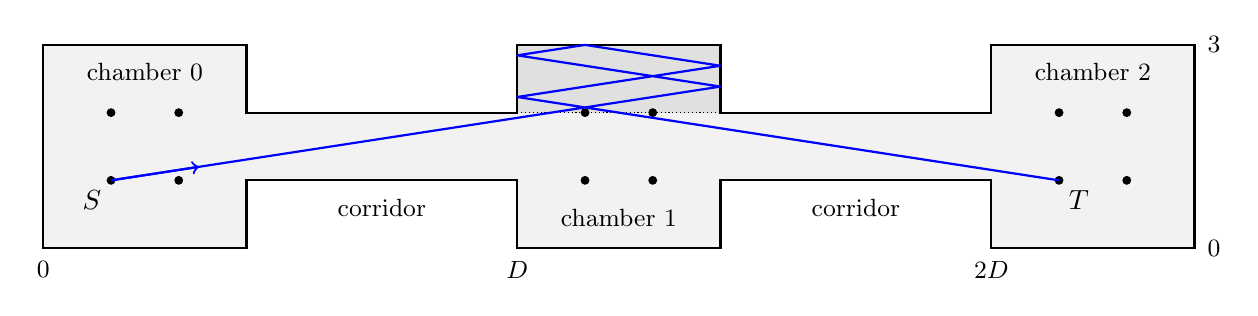
\begin{tikzpicture}[x=0.86cm,y=0.86cm]
  \fill[black!5] (0,0)--(3,0)--(3,1)--(7,1)--(7,0)--(10,0)--(10,1)--(14,1)--(14,0)--(17,0)--(17,3)--(14,3)--(14,2)--(10,2)--(10,3)--(7,3)--(7,2)--(3,2)--(3,3)--(0,3)--cycle;
  \fill[black!12] (7,2) rectangle (10,3);
  \draw[thick] (0,0)--(3,0)--(3,1)--(7,1)--(7,0)--(10,0)--(10,1)--(14,1)--(14,0)--(17,0)--(17,3)--(14,3)--(14,2)--(10,2)--(10,3)--(7,3)--(7,2)--(3,2)--(3,3)--(0,3)--cycle;
  \draw[densely dotted] (7,2)--(10,2);
  \foreach \x in {1,2,8,9,15,16}{\foreach \y in {1,2}{\fill (\x,\y) circle (1.6pt);}}
  \draw[blue,thick,line join=round]
    (1,1)--(7.5,2)--(10,2.3846)--(7,2.8462)--(8,3)--(10,2.6923)--(7,2.2308)--(8.5,2)--(15,1);
  \draw[blue,->,thick] (1,1)--(2.3,1.2);
  \node[below left] at (1,1) {$S$};
  \node[below right] at (15,1) {$T$};
  \node at (1.5,2.6) {\small chamber 0};
  \node at (15.5,2.6) {\small chamber 2};
  \node at (8.5,0.45) {\small chamber 1};
  \node at (5,0.6) {\small corridor};
  \node at (12,0.6) {\small corridor};
  \node[right] at (17.05,0) {\small $0$};
  \node[right] at (17.05,3) {\small $3$};
  \node[below] at (0,-0.05) {\small $0$};
  \node[below] at (7,-0.05) {\small $D$};
  \node[below] at (14,-0.05) {\small $2D$};
\end{tikzpicture}
\caption{The room $T_1$ ($k=1$, $D=7$, area 35) with its twelve interior
lattice marks. The blue path joins the equal-offset pair $S=(1,1)$ and
$T=(2D+1,1)$. It leaves the band at $(D+\tfrac12,2)$, enters the upper pocket
(shaded), meets the side walls $2k+2=4$ times and the roof once at
$(D+1,3)$, and returns to the band at $(D+\tfrac32,2)$ moving right.}
\label{fig:room}
\end{figure}

\subsection{Proof of Proposition~\ref{prop:reversal}}
\emph{One reversal.} A path with exactly one horizontal reversal consists of two
pieces that are monotone in $x$. If it starts leftward, the reversal lies left
of the source, and the only vertical wall there is $x=0$. If it ends leftward,
the reversal lies right of the target, at $x=2D+3$. Unfold at that wall and
unfold all reflections at horizontal walls. Horizontal walls lie on integer
lines, so every unfolded image of the row $y=1$ is an odd integer, and the
ordinate halfway along the unfolded straight segment is an integer.

For a left reversal, represent the source at $-u$; the midpoint abscissa is
$(-u+2D+u)/2=D$. For a right reversal, represent the target at
$2(2D+3)-(2D+u)$; the midpoint abscissa is $D+3$. Unfolded abscissas in
$[0,2D+u]$ in the left case, or $[u,2D+3]$ in the right case, are actual
abscissas, because the fold at the reversal wall is the identity on the forward
side (review correction 1 of \cite{d200}). Since $0<D<D+3<2D+3$, the midpoint
lies on the physical rightward pass through a mouth of the middle chamber.
Refolding the horizontal reflections preserves integrality, so the path
crosses that mouth at an integral height. The open aperture is $1<y<2$, which
contains no integer. This rules out one reversal.

\emph{Zero reversals.} The midpoint abscissa is $D+u$. Take $u=1$. In the
vertically unfolded middle chamber, the straight segment has an integral
ordinate $m$ one unit after entry. The global and middle-chamber vertical
coordinates differ by a composition of reflections in integer lines, hence by
$y\mapsto\pm y+2m'$ with $m'\in\Z$, so $m$ is an integer (review correction 2 of
\cite{d200}). If $a,b$ are the unfolded ordinates at the two mouths, then
$b=a+3(m-a)=3m-2a$. Middle-chamber folds have period 6 and preserve
$(1,2)\cup(4,5)\bmod 6$, which is $(1,2)\bmod 3$; both $a$ and $b$ must lie in
this set. Write $a=3t+1+\varepsilon$ with $0<\varepsilon<1$. Then
$b\equiv 1-2\varepsilon\pmod 3$, which lies in $(0,1)$ for
$\varepsilon<\tfrac12$, equals $0$ at $\varepsilon=\tfrac12$, and lies in
$(2,3)$ for $\varepsilon>\tfrac12$. It is never in $(1,2)$. The map
$x\mapsto 2D+3-x$ together with path reversal exchanges the offsets $1$ and
$2$. \qed

\begin{remark}
The review observes that this argument does not use $D\equiv 1\pmod 3$. For
every equal corridor length, the equal-offset outer pair needs at least two
horizontal reversals \cite{d200}.
\end{remark}

\subsection{Proof of Theorem~\ref{thm:three}}
By the vertical reflection $y\mapsto 3-y$, it suffices to treat pairs in which
every same-row mark lies on row $1$.

\emph{Same chamber.} Each chamber is a convex square, so the straight segment
works.

\emph{Different rows, different chambers.} The open segment from row 1 to row 2
stays in $1<y<2$, so it crosses each chamber wall inside an aperture.

\emph{Same row, adjacent chambers.} Bounce once at the opposite corridor wall
$y=2$ at the horizontal midpoint. In local coordinates with the left chamber at
$[0,3]$, that midpoint is $(D+u+v)/2$. It lies strictly between $3$ and $D$
because $D>4$; the review records the exact condition
$D>\max(6-u-v,u+v)$ \cite{d200}. The two halves have opposite vertical slopes
and lie in the open band.

\emph{Same row, outer chambers, distinct offsets $u\ne v$.} Put $H=2D+v-u$,
which is odd. Use increasing horizontal travel $t$ from $0$ to $H$ and the
unfolded ordinate $f(t)=1+3t+t/H$. In a chamber, fold $f$ into $[0,3]$ by
reflection; in a corridor, fold it into $[1,2]$. The two prescriptions join with
equal height and velocity at every seam. Each seam ($x=3$, $D$, $D+3$, $2D$) has
integral $t$, and $z=1+t/H$ lies strictly between $1$ and $2$ there. At even $t$
the shift $3t$ is a period of both folds, so both give $z$ with positive
derivative. At odd $t$ both give $3-z$ with negative derivative: the chamber
shift is $3\bmod 6$ and the corridor shift is $1\bmod 2$. Every mouth is
therefore crossed transversely in its interior. Wall hits between seams occur
where $f(t)$ is an integer and are not at seams, so they are smooth. At $t=H$
the unfolded ordinate is $2+3H\equiv 5\pmod 6$, which folds to $1$ in the last
chamber, the specified target. The path has no horizontal reversal.

For comparison, the pair $(u,v)=(2,1)$ also has a path with exactly one
reversal: unfold the source to $-2$ and bounce at height $2$ at
$x=D-\tfrac12$ in the first corridor. The reflection at $x=0$ is smooth.

\emph{Same row, outer chambers, equal offsets.} This is the pair of
Proposition~\ref{prop:reversal}. Set $L=D-\tfrac12$. Start at $(u,1)$ moving
right and up with slope $1/L$, and use accumulated absolute horizontal travel as
the parameter. The path has four legs, each of horizontal travel $L$, with a
single reversal of vertical velocity at the roof.
\begin{enumerate}
\item The first leg stays in the open band. At $x=3$ its height is
$1+(3-u)/L$, and at $x=D$ it is $1+(D-u)/L<2$. It reaches height $2$ at
$x=D+u-\tfrac12$, inside the middle chamber, so it clears both ends of the first
corridor.
\item Above height $2$ the middle chamber has reflecting sides at local
abscissas $0$ and $3$. The leg starts there at local abscissa
$a=u-\tfrac12$. Unfold the sides. After travel $L$ the ray reaches the roof
$y=3$ at unfolded abscissa $a+L=D+u-1$. Since $D\equiv 1\pmod 3$, this is
congruent to $u\not\equiv 0\pmod 3$, so the ray misses both roof corners.
Reflect at the roof.
\item After another travel $L$ the ray returns to height $2$ at unfolded local
abscissa $a+2L=a+6k+7\equiv a+1\pmod 6$. Because $0<a+1<3$, folding gives local
abscissa $u+\tfrac12$ with rightward velocity. The side contacts are at the
positive multiples of $3$ strictly between $a$ and $a+2L$. Neither endpoint is a
multiple of $3$, so every side contact lies strictly between heights $2$ and
$3$ and none is at a corridor-end corner $(D,2)$ or $(D+3,2)$. There are
$2k+2$ such contacts, an even number, consistent with the rightward exit.
\item The ray continues right and down for travel $L$. It leaves height 2 at
$x=D+u+\tfrac12$; at $x=D+3$ and at $x=2D$ its heights lie strictly between $1$
and $2$. It ends at height $1$ and abscissa $D+u+\tfrac12+L=2D+u$, the target.
\end{enumerate}
These four legs form one billiard trajectory: in the full unfolding the slope
stays $1/L$. Only smooth walls are used. The construction is a formula in $k$
with no bound on denominators.

The five cases (same chamber; different rows; adjacent chambers, same row;
outer chambers, same row, distinct offsets; outer chambers, same row, equal
offsets) and the row symmetry cover all $66$ unordered pairs. \qed

\begin{remark}[Where the hypotheses enter]
The proof uses equal corridor lengths, aligned unit apertures, $3\times 3$
chambers, and $D\equiv 1\pmod 3$. The congruence enters only in the
equal-offset case. The review notes that for $D\equiv 0\pmod 3$ the offset-1
pocket ray hits a roof corner, and for $D\equiv 2\pmod 3$ it leaves the pocket
moving left \cite{d200}. No step uses $W\le 20$ as an inequality.
\end{remark}

\section{The pocket lemma}\label{sec:pocket}
\begin{figure}[t]
\centering
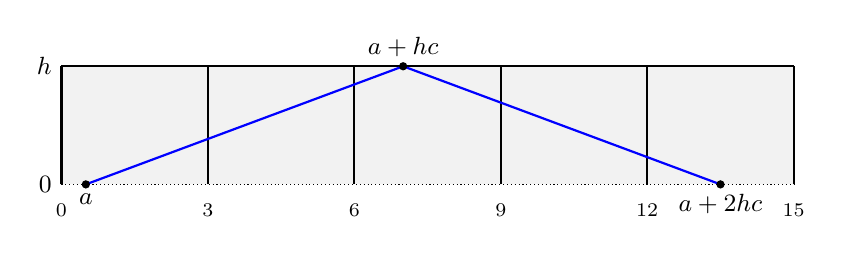
\begin{tikzpicture}[x=0.62cm,y=1.5cm]
  \foreach \i in {0,1,2,3,4}{\fill[black!5] (3*\i,0) rectangle (3*\i+3,1);}
  \foreach \x in {0,3,6,9,12,15}{\draw[thick] (\x,0)--(\x,1);}
  \draw[thick] (0,1)--(15,1);
  \draw[densely dotted] (0,0)--(15,0);
  \draw[blue,thick] (0.5,0)--(7,1)--(13.5,0);
  \fill (0.5,0) circle (1.5pt) node[below] {\small $a$};
  \fill (7,1) circle (1.5pt) node[above] {\small $a+hc$};
  \fill (13.5,0) circle (1.5pt) node[below] {\small $a+2hc$};
  \foreach \x in {0,3,6,9,12,15}{\node[below] at (\x,-0.08) {\scriptsize $\x$};}
  \node[left] at (0,1) {\small $h$};
  \node[left] at (0,0) {\small $0$};
\end{tikzpicture}
\caption{The pocket with its side walls unfolded, drawn for $w=3$, $h=1$,
$a=\tfrac12$ and $c=\tfrac{13}{2}$, the case $k=1$, $u=1$ of
Figure~\ref{fig:room}. The return phase $a+2hc=\tfrac{27}{2}$ is
$\tfrac32\bmod 6$, so the ray leaves at local abscissa $\tfrac32$ moving right.}
\label{fig:unfold}
\end{figure}

\begin{lemma}[Pocket return map]\label{lem:pocket}
Let a pocket occupy $(0,w)\times(0,h)$ with its mouth on $y=0$. A ray enters at
a regular mouth point $a$, moving up and right with $c=|dx/dy|>0$. Then it meets
the roof at unfolded horizontal coordinate $a+hc$ and returns to the mouth at
$a+2hc$. On the phase circle $\R/2w\Z$ the pocket translates the oriented phase
by $2hc$ and reverses the vertical velocity. The excursion is legal if and only
if $a+hc\notin w\Z$ (roof corner), $a+2hc\notin w\Z$ (mouth endpoint), and the
return lies in the actual open part of the mouth. For a leftward start, use the
incoming phase $-a$.
\end{lemma}

\begin{proof}
Unfold the two side walls. The pocket becomes the strip $\R\times(0,h)$ and the
ray is a straight segment with horizontal coordinate $a+c\cdot(\text{vertical
travel})$. It meets the roof at $a+hc$ and returns at $a+2hc$. Folding has
period $2w$ (Section~\ref{sec:setup}), so the return phase records both the
folded position and the horizontal sign. Side hits occur at unfolded multiples
of $w$ strictly between $a$ and $a+2hc$; such a hit is at a corner only if it
coincides with the roof contact or the return. The start $a$ lies in $(0,w)$,
so it is not a multiple of $w$ \cite{R2,d201}.
\end{proof}

Figure~\ref{fig:unfold} shows the unfolded strip.

\subsection{Matching a source and a target}
Suppose the pocket mouth $(0,w)$ lies above a clear horizontal band of height
$g$. Place the source and target on the lower edge of that band at local
abscissas $U$ and $V$, moving right on approach and departure. The open approach
and departure legs must lie in the room, and the marks must be interior points.
The coordinates may also be images obtained by unfolding a known smooth outer
wall. Put $M=U+V$.

\begin{proposition}[Matching criterion]\label{prop:match}
For a full mouth, a legal path consisting of a straight band leg from the source
to entry point $a$, one roof excursion, and a straight band leg from the return
point $b$ to the target exists if and only if
\[
\max(0,\,M-w,\,U)<a<\min(w,\,M),\qquad
\Bigl(2+\frac{2h}{g}\Bigr)a\equiv M+\frac{2h}{g}U\pmod{2w}.
\]
Solutions in $a$ are spaced by $wg/(g+h)$. An open interval of admissible $a$
that is longer than this spacing contains a solution. For a partial mouth,
additionally require $a$ and $M-a$ to lie in the actual opening.
\end{proposition}

\begin{proof}
The two straight band legs force $c=(a-U)/g$ and $b=V-gc=M-a$. Entry and return
in the open mouth mean $0<a<w$ and $0<M-a<w$, and $c>0$ means $a>U$; together
these give the interval. The return condition of Lemma~\ref{lem:pocket} is
$a+2hc\equiv b\pmod{2w}$; substituting $c$ gives the congruence. Because
$b\in(0,w)$, the congruence puts the return phase on the rightward half, so the
exit is rightward. Adding $a$ to both sides gives $2(a+hc)\equiv M\pmod{2w}$, so
$a+hc\equiv M/2\pmod w$; a roof corner would need $M\in 2w\Z$, which
$0<M<2w$ excludes. The mouth-endpoint exclusion holds because $b\notin w\Z$.
Conversely, any legal path with these two legs and one excursion determines $c$
and $b$ as above and so satisfies both conditions. The coefficient of $a$ is
$2(g+h)/g$, so solutions are spaced by $2w\cdot g/(2(g+h))=wg/(g+h)$. An
interval exactly as long as the spacing may contain solutions only at its
endpoints, so strict length is the right condition \cite{R2,d201}.
\end{proof}

An explicit solution is the first progression value strictly above the lower
endpoint, obtained by one floor operation. The criterion depends on the pocket
dimensions, the corridor distances and the mark offsets. A nonzero shift alone
does not guarantee matching. The itinerary can reverse horizontal velocity inside
the pocket, so a midpoint obstruction derived for monotone transits, such as
Proposition~\ref{prop:reversal}, does not apply to it.

\subsection{Independent corridor lengths}
\begin{theorem}[Aligned three-chamber rooms]\label{thm:unequal}
Take three $3\times 3$ chambers $[s,s+3]\times[0,3]$ at $s=0,\,D_1,\,D_1+D_2$,
joined by unit corridors at $1<y<2$, with integers $D_1,D_2\ge 4$ chosen
independently. Every pair of distinct interior lattice marks is lit.
\end{theorem}

The corridor lengths are $X=D_1-3$ and $Y=D_2-3$, so the theorem covers all
$X,Y\ge 1$ with no congruence condition. Each room has $W=20$ and twelve
interior lattice marks.

\begin{proof}
Write $P=D_1+D_2$ and $\Delta=D_2-D_1$. The open band $(0,P+3)\times(1,2)$ lies
in the room, so every band leg below is legal (review correction 3 of
\cite{d201}). Same-chamber pairs connect directly. Different-row pairs connect by
an open segment in the band. Reflect vertically to put the remaining pairs on
row 1.

\emph{Outer chambers.} Let $u,v$ be the source and target offsets. First try a
bounce at height 2 after a smooth reflection at an outer wall. Reflect the source
to $-u$ across $x=0$. The bounce midpoint, relative to the middle chamber's left
face, is $(\Delta+v-u)/2$. If this is negative, the bounce lies in the first
corridor; its absolute position $(P+v-u)/2$ exceeds $3$ because $P\ge 8$.
Alternatively reflect the target across $x=P+3$; the midpoint relative to the
middle chamber is $3+(\Delta+u-v)/2$. If this exceeds $3$, the bounce lies in the
second corridor; its absolute position $(P+6+u-v)/2$ is less than $P$. Neither
case hits a corridor endpoint. Both outer-wall hits are at heights in $(1,2)$,
so they are regular.

If neither strict test holds, then $u-v\le\Delta\le v-u$. Equal offsets give
$\Delta=0$; otherwise $(u,v)=(1,2)$ and $\Delta\in\{-1,0,1\}$. Use the upper
pocket of the middle chamber with $w=3$, $h=g=1$, $U=u-D_1$ and $V=D_2+v$. Then
$M=\Delta+u+v\in\{2,3,4\}$. Since $U<0$, the entry interval is
$(\max(0,M-3),\min(3,M))$, of length $\min(M,6-M)\ge 2$, which exceeds the
spacing $\tfrac32$. The pocket's flanks $x=D_1$ and $x=D_1+3$ are solid on
$[2,3]$ and its mouth is open. Proposition~\ref{prop:match} gives a regular
rightward return, and the second band leg reaches the target.

\emph{Adjacent chambers.} Let $D$ be their spacing. The opposite-edge bounce at
local abscissa $(D+u+v)/2$ lies strictly in the corridor if and only if
$D>\max(6-u-v,\,u+v)$. For $D\ge 4$ this fails only when $D=4$ and $u=v$.
Reverse the room and the path, if necessary, so the pair lies in the first two
chambers; the map $x\mapsto P+3-x$ keeps $u=v$. Unfold the source at the left
outer wall and use the upper pocket of the first chamber with $U=-u$ and
$V=4+u$. Then $M=4$ and the entry interval is $(1,3)$, of length $2>\tfrac32$.
Explicitly, $a=(5-u)/2$ is the first criterion value above $1$; the exit is
$b=4-a$, the roof contact $2a+u=5$ is not a multiple of $3$, and the $x=0$ hit
is at height $1+u/(a+u)\in(1,2)$. The outgoing leg reaches the second chamber.
\end{proof}

\begin{remark}[Agreement with Theorem~\ref{thm:three}]
For $D_1=D_2=3k+4$ the first criterion value is $a=u-\tfrac12$, which is the
pocket ray of Theorem~\ref{thm:three}. The review's check confirms this in all
16 tested cases \cite{d201}.
\end{remark}

\subsection{Local pockets, the reflex budget and R22}
Every strictly simple orthogonal room has a local rectangular return region.
Take a topmost horizontal wall $[x_0,x_1]$ at height $y_{\max}$, and let $y_2$
be the next lower wall height. A vertical wall crossing a height in
$(y_2,y_{\max})$ must end at $y_{\max}$, so $(x_0,x_1)\times(y_2,y_{\max})$ is
interior with solid flanks. Its height can be less than $1$. Such a region gives
a return map at any wall count but supplies no through corridor or band legs
\cite{R2,d201}.

In the aligned three-chamber layout each strictly inset corridor contributes four
reflex shoulders, so at most two fit at $W\le 20$. The review adds that a corridor
flush with a chamber wall costs only two reflex corners, so flush necks are not
bounded by this count (review correction 2 of \cite{d201}). The count does not
force two necks, alignment, or phase matching.

\emph{R22 control.} In the closed dark base room R22, every physical lattice
point with both coordinates odd is a corner \cite{d154}. This excludes an
integral full-mouth pocket of width at least $3$ and height at least $1$: its open
horizontal span would contain an odd integer, its closed vertical span would
contain an odd integer, and the resulting point would be interior, an open-mouth
point, or a smooth roof point. The review notes that the word ``integral'' can be
dropped, because a pocket with a fractional mouth and height at least $1$
contains an integral one \cite{d201}. The argument does not exclude narrower or
partial pockets. R22 has $W=22$, so this is a control, not a statement about
$W\le 20$.

\subsection{Two-neck words and displaced apertures}
Insert a strictly inset rectangular neck from one side of a rectangle to an end
chamber. Traced counterclockwise, the boundary gains $F=\mathrm{RRLLLLRR}$. For
two attachments the cyclic word is $F\,\mathrm{L}^j\,F\,\mathrm{L}^{4-j}$, where
$j\in\{0,1,2\}$ counts middle-chamber corners on one arc between the attachments
\cite{R3,d201}.

\begin{center}
\begin{tabular}{lcl}
\toprule
Mouths on the middle chamber & $j$ & Word (least rotation or reversal)\\
\midrule
Opposite sides (the family above) & 2 & \texttt{LLLLRRLLRRLLLLRRLLRR}\\
Adjacent sides & 1 & \texttt{LLLLRRLLLRRLLLLRRLRR}\\
Same side & 0 & \texttt{LLLLRRLLLLRRLLLLRRRR}\\
\bottomrule
\end{tabular}
\end{center}

A turn word records no alignment of nonconsecutive walls. A theorem for every
rectangular assembly would still need a realization argument to cover a word.

\begin{lemma}[Displaced strip transit]\label{lem:strip}
Let the middle chamber occupy $0<x<w$, with the left neck opening at heights
$(l_1,r_1)$ and the right neck at $(l_2,r_2)$, where $\delta=l_2-r_1>0$. Take
$S=(U,r_1-g_1)$ in the left outer chamber and $T=(V,l_2+g_2)$ in the right outer
chamber, with $U<0$, $V>w$ and $g_1,g_2>0$, and assume the straight exterior
legs clear their corridors (for example $g_1\le r_1-l_1$ and
$g_2\le r_2-l_2$). A path with these straight legs and one bottom-to-top
transit of the strip $r_1<y<l_2$ exists if and only if
\[
\max\Bigl(0,\,-\frac{U}{g_1},\,\frac{V-w}{g_2}\Bigr)<c<
\min\Bigl(\frac{w-U}{g_1},\,\frac{V}{g_2}\Bigr),\qquad
(g_1+\delta+g_2)\,c\equiv V-U\pmod{2w}.
\]
\end{lemma}

\begin{proof}
The strip has solid flanks, because each side of the middle chamber has one
aperture. A ray entering at $a$ moving up and right exits at phase
$a+\delta c\bmod 2w$, the one-pass version of Lemma~\ref{lem:pocket}. Entry and
exit are $a=U+g_1c$ and $b=V-g_2c$. The inequalities put both contacts inside
the middle chamber, and the congruence matches $b$ on the rightward sheet.
Unfolding the middle flanks glues the three legs with one slope
\cite{R3,d201}.
\end{proof}

An open interval longer than $2w/(g_1+\delta+g_2)$ guarantees a solution. For
$g_1=g_2=1$, write $A=-U$ and $K=V-w$. The interval has length $w-|A-K|$, so
$|A-K|<w\delta/(\delta+2)$ suffices, uniformly in the corridor lengths and chamber
dimensions; the review notes that $A=K$ works for every $\delta>0$ \cite{d201}.
If $|A-K|\ge w$ the interval is empty. A straight leg through a unit neck of
length $L$ has $|dy/dx|<1/L$; it cannot also reach the upper pocket at or above
the top of the right unit mouth when $(\delta+1)L\ge w$ (the source states this
sharp form after the review). The review states the reflected lower-pocket
obstruction from the right as $\delta L_2\ge w$ \cite{d201}. These obstructions
concern the prescribed legs only. They do not exclude exterior wall bounces,
other middle itineraries, or illumination.

\begin{remark}[The word does not force the comparison pocket]
For every integer $H\ge 5$, take three chambers of width $1$ and height $H$ with
two length-one necks at heights $(1,H-1)$. Each neck is strictly inset at both
ends, giving the opposite-side word. No integral full-mouth pocket of width at
least $3$ and height at least $1$ exists anywhere in this family \cite{R3}; the
review's script confirms this for $H=5,6,9$ \cite{d201}. The family is not
claimed to be lit.
\end{remark}

\section{Neck phase maps}\label{sec:neck}
This section lets the exterior legs reflect inside unit necks. Take the middle
chamber at $0<x<w$ with floor strictly below $0$, so the left neck is strictly
inset. Its left opening is $(0,1)$ in height and its right opening is
$(1+\delta,2+\delta)$ with integral $\delta>0$. The middle roof is $h>0$ above
the upper opening. Let $S$ lie in the left outer chamber at height $0$ and $T$
in the right outer chamber at height $\delta+2$. Their horizontal distances to
the outer neck mouths are $e$ and $f$, and the neck lengths are $L$ and $R$.
Write $A=e+L$, $K=f+R$ and $r=|dy/dx|$ \cite{R4}.

\begin{lemma}[Neck map]\label{lem:neck}
Launch $S$ up and right, trace backward from $T$ down and left, and require
$er<1$ and $fr<1$ for straight outer stubs. Measured up from the lower left-neck
wall and down from the upper right-neck wall, the unfolded phases at the middle
chamber are $Ar$ and $Kr$ modulo $2$. A residue $z\in(0,1)$ folds to depth $z$
with the launch sign, and $z\in(1,2)$ folds to depth $2-z$ with the opposite
sign. Integral phases hit mouth endpoints and are excluded. Every intervening
neck-wall bounce is smooth.
\end{lemma}

\begin{proposition}[Coupled slope formulas]\label{prop:slopes}
Let $i,j,m\ge 0$ be integers.
\begin{enumerate}
\item \emph{Displacement strip.} Let $\alpha=Ar-2i$ and $\beta=Kr-2j$ lie in
$(0,1)$. A path entering the middle chamber at height $\alpha$, crossing the
strip, and leaving at height $\delta+2-\beta$ exists exactly when
\[
r=\frac{\delta+2+2i+2j}{A+K+(2m+1)w},
\]
with $er,fr<1$ and $1-\alpha,\,1-\beta<wr$.
\item \emph{Upper roof pocket.} Let $0<\alpha=Ar-2i<1$, $1<Kr-2j<2$ and
$\beta=2j+2-Kr$. A path with one roof excursion exists exactly when
\[
r=\frac{\delta+4+2i+2j+2h}{A+K+(2m+1)w},
\]
with $er,fr<1$ and $\delta+2-\alpha<wr$, $\beta<wr$.
\end{enumerate}
\end{proposition}

\begin{proof}
For the strip, the entry reaches height $1$ at $a=(1-\alpha)/r$, and the
backward trace reaches height $1+\delta$ at $b=w-(1-\beta)/r$. The conditions
$a,b\in(0,w)$ keep the two short end pieces free of side contacts. The full
vertical sides are solid between those levels, and the translation
$a+\delta/r\equiv b\pmod{2w}$ joins the pieces. The total unfolded horizontal
travel across the middle rectangle is $(2m+1)w$, and $2m$ side reversals leave
the exit rightward; solving gives the first formula. For the roof, the legs
require $a=(\delta+2-\alpha)/r$ and $b=w-\beta/r$, and the excursion translates
$a$ by $2h/r$ modulo $2w$. Roof clearance follows from
$2(a+h/r)\equiv a+b\pmod{2w}$ with $0<a+b<2w$, as in
Proposition~\ref{prop:match} \cite{R4,d202}.
\end{proof}

\paragraph{Explicit families.} With $e=f=1$ and $r=\tfrac12$:
\begin{itemize}
\item Take $w=2$, $\delta$ any positive even integer, and $L,R$ positive
multiples of $4$. Both phases are $\tfrac12$, so $a=b=1$, and the strip adds
$2\delta$, a multiple of $2w$. The marks connect even when $|A-K|$ is large
enough to make the direct-leg interval of Lemma~\ref{lem:strip} empty.
\item Take any integral $\delta\ge 1$, $w=2\delta+8$, $h=\delta+5$, $L$ a
positive multiple of $4$ and $R\equiv 2\pmod 4$. The neck residues are
$\tfrac12$ and $\tfrac32$, $a=2\delta+3$ and $b=2\delta+7$. The roof shift
$4h=2w+4$ gives the required four-unit displacement. The roof contact
$4\delta+13$ is odd, so it is not a multiple of $w$ \cite{d202}.
\end{itemize}

\begin{proposition}[A joint obstruction for straight stubs]\label{prop:K2A}
Suppose the data are integral, $K=2A$ and $\max(e,f)\ge 3w$. Both tests of
Proposition~\ref{prop:slopes} fail for every admissible slope of the straight
stubs, however many bounces occur in either neck.
\end{proposition}

\begin{proof}
Straight stubs need $er,fr<1$, so $wr<\tfrac13$. The strip test needs
$1-\alpha<\tfrac13$, so $\alpha>\tfrac23$; then $Kr\equiv 2\alpha\pmod 2$ lies in
$(\tfrac43,2)$, on the wrong sheet. The roof test needs
$\delta+2-\alpha<wr<\tfrac13$, but $\delta+2-\alpha>2$ \cite{R4,d202}.
\end{proof}

The obstruction occurs with arbitrarily long necks, for example $e=f=3w$ and
$R=2L+3w$. It is not evidence that the marks are dark.

\paragraph{Arbitrary outer chambers.} In a rectangular outer chamber with floor
$F$, height $H_0$ and width $W_0$, unfold its horizontal walls before folding the
neck. For a source at height $y$ moving horizontally toward its neck at distance
$e$, launched with vertical sign $\sigma$, the chamber phase at the neck is
$y-F+\sigma er\bmod 2H_0$. Fold into $[0,H_0]$, add $F$, and multiply $\sigma$ by
the sign of the fold's derivative. Require the height to lie strictly inside the
aperture $(l,l+g)$, where $g$ is the aperture height. If the height above $l$ is
$z$, start the neck at phase $z$ for an upward arrival or $-z$ for a downward one.
A neck of length $L$ advances the phase by $Lr\bmod 2g$; a return at phase $0$
or $g$ hits a mouth endpoint. The same rule, run backward from $T$, handles
independent outer dimensions. If the outer wall opposite the mouth is solid, a
single initial horizontal reversal replaces $e$ by $2W_0-e$, after checking that
the wall contact misses a corner \cite{R4}.

For unit displaced necks with physical entrance heights $y_L,y_R$ and right/up
forward velocity on the left, the strip test reads $(2m+1)wr=y_R-y_L$ with
$0<1-y_L<wr$ and $0<y_R-(\delta+1)<wr$. The roof test, with a right/down
continuation, reads $(2m+1)wr=2Y-y_L-y_R$ with $Y=\delta+2+h$,
$0<\delta+2-y_L<wr$ and $0<\delta+2-y_R<wr$ \cite{R4}.

\paragraph{A reflected-stub connection in the $K=2A$ residual.} Take
$r=\tfrac14$ and independent integral outer heights $H_0,H_1$ large enough for
strictly inset apertures. Choose $e=8H_0i+1$ and $f=8H_1j+1$ with positive
integers $i,j$, in sufficiently wide end chambers. Take $L$ a positive multiple
of $8$ with $2L>f-2e$, set $A=e+L$ and $R=2A-f>0$. Then $K=2A$ and the middle
entrance phases are $\tfrac14$ and $\tfrac12$. Choose $w\equiv 1\pmod 4$,
$w\ge 5$, and $\delta=((4n+1)w-5)/4$ with an integer $n\ge 1$. The strip test
holds with $m=2n$: the unfolded rise is $\delta+\tfrac54=(4n+1)w/4$. This works
with $e,f\ge 3w$, where Proposition~\ref{prop:K2A} rules out straight stubs.
The source states the condition on $L$ after review correction 4 of
\cite{d202}.

\paragraph{Adjacent mouths.} For a left entrance $(l,l+1)$ and a top exit
$(t,t+1)$ in a middle rectangle $[0,w]\times[0,H]$, the two phases advance by
$Lr$ and $R/r$. A middle leg with no wall hit from $(0,y)$ moving up and right
to $(x,H)$ exists exactly when $x=(H-y)/r$ with both mouth coordinates strictly
interior. With $r=\tfrac23$: put $S$ one unit left of the outer left-neck mouth
at height $l$, take $L$ a positive multiple of $3$, choose $H-l$ an odd integer
at least $3$, $t=3(H-l-1)/2$ and $w>t+1$. Put $T$ one unit beyond the far end of
the top neck at transverse coordinate $t+2$, and take $R$ a positive multiple of
$4$. The ray reaches $(0,l+\tfrac23)$ and $(t+\tfrac12,H)$, giving a legal
connection with unbounded lengths on both axes \cite{R4,d202}. This family does
not cover arbitrary adjacent-side pairs.

\subsection{A lit family with a \texorpdfstring{$3\times 4$}{3 x 4} middle chamber}
\begin{theorem}[Tall middle chamber]\label{thm:tall}
Take end chambers $[0,3]\times[0,3]$ and $[P,P+3]\times[0,3]$, a middle chamber
$[D_1,D_1+3]\times[0,4]$, and unit necks at $1<y<2$ with independent lengths
$X,Y\ge 1$, so $D_1=X+3$, $D_2=Y+3$ and $P=D_1+D_2$. Every pair of distinct
interior lattice marks is lit.
\end{theorem}

Each room has $W=20$, the opposite-side word, and 14 interior lattice marks,
giving 91 pairs. At $X=Y=1$ the area is 32 \cite{d202}.

\begin{proof}
\emph{Rows 1 and 2.} The direct segments and adjacent corridor bounces of
Theorem~\ref{thm:unequal} are unchanged; the adjacent length-one exception uses
the pocket of the $3\times 3$ end chamber. The outer-wall reflection tests depend
only on horizontal coordinates. In the remaining cases $M\in\{2,3,4\}$ and the
open entry interval has length at least $2$. For row 1 the upper middle pocket
now has $h=2$, $w=3$, $g=1$, with spacing $1$. For row 2 use the lower pocket
beneath height $1$, of depth $1$, by reversing the vertical coordinate; its
spacing is $\tfrac32$. Both fit strictly.

\emph{Row 1 to the middle row 3.} Put the pocket base at height 2 with width $w$
and height $h$, and the middle target at local abscissa $v\in(0,w)$ and height
$2+t$, $0<t<h$. Orient $x$ so the source abscissa $U$ is negative. From $S$ at
height 1 go right and up to the base at $a=U+c$, in the open band. Unfolding only
the sides gives the exact condition
\[
0<a<w,\qquad (1+t)a\equiv \pm v+tU\pmod{2w}.
\]
For integral $t\ge 1$ each sign has spacing $2w/(1+t)\le w$. When equality holds
the two residues differ, since $0<v<w$, so they cannot both lie only at
endpoints. One legal $a$ exists, and all side contacts lie strictly between the
base and the roof.

\emph{Row 2 to the middle row 3.} Orient $x$ from the outer source, let
$v\in\{1,2\}$ be the target's distance from the middle entrance, and let $B$ be
the full horizontal separation. Put $m=2/v$ and use the unfolded ordinate
$2+6mx-x/B$ at horizontal travel $x$ from $S$. At every integral seam before the
middle chamber, $6mx$ is a multiple of the end-chamber period $6$ and the neck
period $2$, and the slow ordinate $2-x/B$ lies in $(1,2)$, so both folds agree in
height and have positive derivative. In the middle chamber, unfold about $0$ and
$4$. The final unfolded height, measured from the entrance copy, is
$1+6mv=13\equiv 3\pmod 8$. There is no later seam, and the target is interior.

Marks inside the middle chamber see one another directly. With reversal
$x\mapsto P+3-x$ these cases exhaust the pairs \cite{R4,d202}.
\end{proof}

\paragraph{A sufficient height condition.} Take an end chamber of integral
height $H_0$ containing the unit band, with floor $F<1$ and $F+H_0>2$, and a middle
chamber with floor $0$ and integral height $H$. For a source at integral abscissa
and a positive integer $m$, the row-2 slope $2H_0m-1/B$ reaches target height $y$
if $2H_0vm\equiv\pm y-1\pmod{2H}$, that is, if $\gcd(2H_0v,2H)$ divides at least
one right-hand side. The integrality of $m$ and the source abscissa, and the
bounds on $F$, are review correction 5 and its gap list in \cite{d202}. The
condition never holds for $y=2$, because $\pm 2-1$ is odd; that row is already
covered by band segments. It fails for row 4 of a $3\times 5$ middle chamber
with $H_0=3$. Failure does not exclude other paths.

\section{The group-ring test}\label{sec:groupring}
Normalize the common band to $0<y<1$. Chamber $i$ has horizontal interval
$(l_i,l_i+w_i)$, floor $-b_i$ and roof $1+t_i$, with $b_i,t_i$ positive integers;
the two gaps between chambers have arbitrary positive integral lengths. A unit
neck has no interior lattice row, so every lattice mark lies strictly inside a
chamber column \cite{R5}.

\paragraph{Strip data.} Use longitudinal travel as time, so a prescribed roof
reflection reverses the physical longitudinal velocity while time keeps
increasing. In piece $j=1,\dots,s$ let $d_j$ be the longitudinal travel and
$(f_j,f_j+B_j)$ the transverse interval, with solid transverse walls, and let the
next gate be the actual open interval $(a_j,b_j)$ through which the ray passes.
All data are integral, and the two marks are lattice points (review correction 3
of \cite{d203}). A roof bounce carries a gate that excludes its two corners. Let
$D=\sum_j d_j>0$, and let $x_0,x_s$ be the transverse coordinates of the marks.
Paths along an axis use the direct segment test separately; below, both absolute
velocity components are positive.

\paragraph{The coefficient $J$.} Choose transverse velocity signs
$\varepsilon_0,\dots,\varepsilon_s$ at the source, gates and target, with the
same sign on both sides of each gate. Form the finite abelian group
\[
G=\Bigl(\prod_{j=1}^{s}\Z/(2B_jD)\Bigr)\Big/\bigl\langle(d_1,\dots,d_s)\bigr\rangle.
\]
In coordinate $j$ put
$E_j=\varepsilon_j(z_j-Df_j)-\varepsilon_{j-1}(z_{j-1}-Df_j)$ with $z_0=Dx_0$
and $z_s=Dx_s$. Write $E=c+\sum_i g_iz_i$ in $G$, with one column $g_i$ for each
intermediate gate. For gate $(a_i,b_i)$ set $L_i=Da_i+1$ and $U_i=Db_i-1$. In the
integral group ring $\Z[G]$, take the coefficient of the identity in
\[
[c]\prod_i[L_ig_i]\bigl(1+[g_i]+\dots+[(U_i-L_i)g_i]\bigr),
\]
where an empty interval gives zero. Let $J$ be the sum of these nonnegative
coefficients over all sign choices. $J$ depends only on the gate and dimension
data; no direction or reflection itinerary is enumerated to define it.

\begin{theorem}[Exactness of the group-ring test]\label{thm:J}
$J>0$ if and only if a legal path through the prescribed sequence of strip
transits exists.
\end{theorem}

\begin{proof}
In each piece the oriented phase advances by $d_jv$ modulo $2B_j$, where $v$ is
the absolute transverse speed per unit longitudinal travel; the endpoint
difference is $E_j/D$. Unfold all reflections. In every reflected copy the map
between physical and unfolded coordinates is $\pm U+c'$ with $c'$ an integer,
since $c'$ starts integral at a lattice mark and each reflection sends $c'$ to
$2\cdot\mathrm{wall}-c'$. So both marks have integral transverse coordinates in
every copy, and $n=Dv$ is an integer. Each gate coordinate times $D$ is then an
integer, and a strict gate $a<z/D<b$ becomes $Da+1\le z\le Db-1$. The quotient in
$G$ eliminates $n$ from the congruences $E_j\equiv d_jn\pmod{2B_jD}$. Conversely,
zero in $G$ supplies a common integer $n$, which can be made positive by adding
a common period. Strict gate intervals give smooth crossings with the specified
signs, and transverse reflections inside a piece cannot land on a gate line.
Folding constructs the ray \cite{R5,d203}.
\end{proof}

The identity $Dv=n$ is an endpoint identity. It is not a bound on the denominator
of a connecting ray, and no bound on the order of $G$ is needed. The review's
script checks, on 12 itineraries, that the group-ring coefficient equals a direct
enumeration, and that all 22 resulting solutions reach the target \cite{d203}.

\paragraph{Itineraries.} The source prescribes a finite list of strip
sequences \cite{R5}. Horizontal tests run through the clipped list of chambers and
necks between the marks, with optional reflections at a solid end wall; they
include necks with any number of vertical reversals. Vertical tests run from a
mark to the band through its chamber column, optionally after a roof or floor
reflection, then cross the band once (marks on opposite sides) or twice with an
intervening neck-wall bounce or chamber excursion (marks on the same side).
The earlier pocket criterion and the gcd lift are special cases. A mixed test
joins two folded neck prefixes through one middle-chamber roof return; it reduces
to deciding whether a monotone rational function of $r$ on each fold piece takes
a positive odd integer value, which endpoint floors decide.

\subsection{Dimension-only consequences}
Let $P$ be the full horizontal span, with the far left wall at $0$.

\begin{corollary}[Opposite-side pairs]\label{cor:opp}
Let $S$ lie on or below the lower band edge and $T$ on or above the upper one, in
different chambers of widths $u,v$. If $\gcd(P,\operatorname{lcm}(u,v))=1$, the
pair is lit, for arbitrary chamber heights, vertical offsets and neck lengths.
\end{corollary}

\begin{proof}
Put $a=-y_S$, $b=y_T-1$, $M=\operatorname{lcm}(2u,2v)$ and $g=\gcd(M,2P)$. Pick a
signed residue $d$ of $x_T-x_S$ modulo $g$ and set $\eta=d/(a+1+b)$. Choose an
arbitrarily large integer $m$ with $Mm\equiv x_T-x_S-d\pmod{2P}$, set
$c=Mm+\eta>0$, and launch up and right. During the first $a$ units of rise the
source chamber folds away $Mma$, a multiple of $2u$, so the ray reaches the band
at $x_S+a\eta$ moving right. The band adds $c$ modulo $2P$, which puts the exit
at $x_T-b\eta$ on the rightward sheet. The last $b$ units of rise end at $T$. This
works whenever $x_S+a\eta$ and $x_T-b\eta$ lie in the open spans of the source and
target chambers. Under the coprimality hypothesis $g=2$, so $|d|\le 1$; then
$|a\eta|,|b\eta|<1$, while an integral interior abscissa is at least one unit from
either flank \cite{R5,d203}.
\end{proof}

More generally, for the least absolute residue $d$, the test
$|d|\max(a,b)<a+1+b$ certifies all horizontal offsets with that residue.

\begin{corollary}[Same-side pairs of opposite parity]\label{cor:same}
If $\gcd(P,\operatorname{lcm}(w_1,w_2,w_3))=1$ and the two mark abscissas have
opposite parity, the pair is lit at arbitrary depths.
\end{corollary}

\begin{proof}[Proof sketch from the source]
Orient vertically so both marks lie on or below the near band edge, at integral
depths $a,b$. Put $M=2\operatorname{lcm}(w_1,w_2,w_3)$ and $\Delta=x_T-x_S=2K+d$
with $K$ even and $d\in\{-1,1\}$. Since $\gcd(M,2P)=2$, choose $m$ with
$Mm\equiv K\pmod{2P}$, positive and large. Unfold the band's end walls to a chain
mirrored every $P$. At $z=x_S+K$ the open unit cell on the side of $d$ is either
entirely neck wall ($h=0$) or entirely above one chamber aperture, leading into a
pocket of height $h$, because all boundaries are integral. With
$\eta=d/(a+2+2h+b)$ and $c=Mm+\eta$, the band contact, the roof contact and the
return all lie strictly inside that cell, and the ray finishes at
$x_S+2K+(a+2+2h+b)\eta=x_T$ modulo $2P$ on the target sheet \cite{R5,d203}.
\end{proof}

\begin{proposition}[Finite exceptional set for odd $P$]\label{prop:exc}
Assume the hypothesis of Corollary~\ref{cor:same} and that $P$ is odd. Let $E$ be
the four internal neck-end abscissas and their negatives modulo $2P$. A
same-side pair of equal-parity abscissas that the zero-drift construction of
\cite{R5} does not light has both parity-compatible midpoint roots $z_\pm$ in $E$,
so $x_S\equiv z_++z_-$ and $x_T\equiv z_+-z_-\pmod P$. At most $8^2=64$ ordered
abscissa pairs remain, independent of widths, heights and corridor lengths.
\end{proposition}

The zero-drift construction uses lifts $X=\pm x_S$, $Y=\pm x_T$ and a midpoint
$z$ with $2z\equiv X+Y\pmod{2P}$, $z\equiv X\pmod 2$, inside a chamber span or a
neck span of the mirrored chain; with $\eta=0$ every integral-depth leg returns to
its own transverse coordinate. For odd $P$ each lift has exactly one root of the
right parity, and no root is $0$ or $P$. The exception is realizable: widths
$4,6,4+156k$ with neck lengths $2,1$ for $k\ge 1$ have internal seams
$4,6,12,13$ and $P=17+156k$, odd and coprime to every width. At $x_S=8$, $x_T=16$
the two roots are $12$ and $-4$, both seams \cite{R5}. This example shows only
that the zero-drift construction misses these abscissas. It does not show that
$J$ or the other tests vanish. In the review's grid of 789 coprime rooms, each of
the 1,218 zero-drift exceptions has a positive $J$ for some itinerary of at most
5 pieces \cite{d203}.

\subsection{Narrow chambers}
\begin{theorem}[Width-two chambers]\label{thm:w2}
Suppose all three chamber widths are $2$, the left neck length is odd and the
right neck length is $2\bmod 4$ (or the reverse). For any positive integral
depths above and below the band, every pair of distinct interior lattice marks is
lit.
\end{theorem}

\begin{proof}
$P$ is odd, hence coprime to every width. Each chamber has one interior abscissa:
$1$, $x=3+L_1$ and $y=x+2+L_2$; the last two are even. Corollaries~\ref{cor:opp}
and~\ref{cor:same} handle all pairs except same-side pairs at $x$ and $y$. Their
midpoint $z=x+(2+L_2)/2$ is even and lies strictly inside the second neck
$(x+1,y-1)$, so a zero-drift return is regular \cite{R5,d203}.
\end{proof}

The area-21 room with three $2\times 3$ chambers and necks of lengths $1$ and $2$
is the case $L_1=1$, $L_2=2$, height $3$; its abscissas are $1,4,8$ and the
decisive midpoint is $6$.

\begin{proposition}[End-pocket test]\label{prop:endpocket}
In coordinates with band $(0,1)$, let $S$ at abscissa $s$ and $T$ at abscissa
$l+v$ lie on the lower band edge, and let the target chamber span $(l,l+w)$ with
lower pocket depth $b$. Choose an integer $0<e<w$, put $x_E=l+e$ and
$c_0=(2P-x_E-s)/2$, and require $s+c_0$, folded into $[0,P]$, to lie strictly
inside a neck span. For $c=c_0+2Pn$ with $n\ge 0$, the ray bounces at the upper
neck wall, returns to the lower edge at $x_E$ moving left, and reaches $T$ after
one floor reflection exactly when
\[
e-2bc\equiv\pm v\pmod{2w},\qquad e-bc\notin w\Z.
\]
The congruence is soluble if and only if $\gcd(4bP,2w)$ divides $e-2bc_0\mp v$ for
at least one sign. A separate corner check is needed only when $e=v$
\cite{R5,d203}.
\end{proposition}

\begin{corollary}[Width-one middle chamber]\label{cor:w1}
Take end widths $3$, middle width $1$, equal neck lengths $L\ge 1$, and all
chamber heights $3$ with the neck centrally inset. Every pair of distinct interior
lattice marks is lit.
\end{corollary}

\begin{proof}
The middle chamber has no interior lattice marks. Different rows connect
directly; by symmetry same-row pairs lie on the lower edge. For distinct outer
offsets the separation $B$ is odd, because the right end starts at $4+2L$; the
unfolded ordinate $3t+t/B$ joins the lower row to itself, as in
Theorem~\ref{thm:three}. For equal offsets take offset $1$ by symmetry, so
$P=7+2L$. Proposition~\ref{prop:endpocket} with $w=3$, $b=1$, $e=2$, $v=1$,
$s=1$ gives $c_0=P/2$, an upper contact $1+P/2$ strictly inside the right neck,
and a lower contact at the interior abscissa $P-1$. The target condition at
$n=0$ is $2-P\equiv\pm 1\pmod 6$, which holds for $L\equiv 0,1\pmod 3$. The review
shows that $n=1$ ($c=5P/2$) gives $2-5P\equiv 1\pmod 6$ for $L\equiv 2\pmod 3$, so
the end-pocket test covers every $L\ge 1$ (review correction 1 of \cite{d203}).
The source instead uses, for $L\equiv 2\pmod 3$, a left outer-wall reflection
followed by an upper corridor bounce at $2+L$, inside the left neck since
$L\ge 2$; that route is also correct. The floor is clear because $e\ne v$.
\end{proof}

The area-23 room (chambers $3\times 3$, $1\times 3$, $3\times 3$, necks of length
$1$) is the case $L=1$.

\paragraph{Height five.} The gcd condition of Section~\ref{sec:neck} misses row-4
targets in a $3\times 5$ middle chamber. The review shows that the coprime
results light these pairs in the named room with chambers $3\times 3$,
$3\times 5$, $3\times 3$ and necks $1,1$ ($P=11$): two by
Corollary~\ref{cor:same} and two by zero drift (review correction 2 of
\cite{d203}).

\subsection{The residual}
For fixed dimensions, a cross-chamber pair escapes the tests of this section
exactly when every group-ring coefficient over the stated itinerary list vanishes
and, for outer pairs, neither mixed roof test contains a positive odd integer on
an admissible interval. The review asks that the itinerary list be named; it is
the horizontal and vertical lists above plus the two mixed branches (review
correction 4 of \cite{d203}). This describes the residual pair by pair. The
source proves neither that the residual is empty nor that any residual pair is
dark. Repeated excursions alternating between pockets could supply further
paths. The aligned layout is therefore not closed by Theorem~\ref{thm:J}.

\section{Scope and limitations}\label{sec:scope}
\paragraph{Review status.} Each main result has one independent AI review:
Theorem~\ref{thm:three} and Proposition~\ref{prop:reversal} in \cite{d200}
(verdict: correct); Lemma~\ref{lem:pocket}, Proposition~\ref{prop:match},
Theorem~\ref{thm:unequal} and Lemma~\ref{lem:strip} in \cite{d201} (correct; the
corner-budget and R22 paragraph is correct with gaps); Section~\ref{sec:neck} in
\cite{d202} (correct with gaps); and Section~\ref{sec:groupring} in \cite{d203}
(correct with gaps). No human referee has checked any of these results, and none
is formally verified.

\paragraph{Gaps recorded by the reviews.} The d200 gaps are the two one-line
justifications in Proposition~\ref{prop:reversal} and the $k\ge 6$ scope; the
source now includes all three fixes. The d201 gaps are the band-leg containment
in Theorem~\ref{thm:unequal}, the flush-neck count, and a broken link; the
manuscript includes the first two. The d202 gaps are the middle floor, a reused
symbol, the condition on $L$ in the reflected-stub family, and the hypotheses of
the height condition; the source fixes the first three and the manuscript states
the last. The d203 gaps are the integral-mark hypothesis, the source chamber in
the gcd lift's modulus, the unneeded $L\equiv 2\pmod 3$ route, a missing
remark on height five, and the unnamed itinerary list. The manuscript states each
fix. No review found an error in a proof step.

\paragraph{Lattice endpoints only.} Every theorem concerns interior lattice
marks. The reviews note that real and rational endpoints are not treated
\cite{d201,d202,d203}, although the pocket criterion itself does not need
lattice marks.

\paragraph{R22 and wall counts.} The 22-wall room R22 does not have the
three-square, aligned-corridor decomposition, so its known dark pair does not
contradict Theorem~\ref{thm:three} \cite{R1}. The results do not imply a
general wall-count bound for dark rooms; in particular they supply no threshold
between eight and nine reflex corners. The opposite-side word
\texttt{LLLLRRLLRRLLLLRRLLRR} is only partly covered: chamber widths and heights,
neck heights, aperture positions and real endpoints remain free \cite{d201,d202}.

\paragraph{What remains open.}
\begin{itemize}
\item \emph{Non-coprime aligned rooms.} No dimension-only theorem is proved when
$\gcd(P,\operatorname{lcm}w_i)>1$. The review's example has chambers
$3\times 3$, $1\times 3$, $2\times 3$ and necks $1,2$ (area 21, gcd 3). Its four
same-row pairs have $J>0$ through a neck bounce, and the traced rays reach the
target; the review did not check its cross-row pairs, so it does not claim the
room is lit \cite{d203}.
\item \emph{Other shapes.} The $4\times 3$ middle chamber, displaced or non-unit
necks, chamber heights other than the aligned band, and general displaced mouths
(including the branch with $\alpha\in(1,2)$) remain open \cite{d202,d203}.
\item \emph{Other words.} The adjacent-side and same-side two-neck words
\texttt{LLLLRRLLLRRLLLLRRLRR} and \texttt{LLLLRRLLLLRRLLLLRRRR} remain open; the
adjacent-side word has one explicit lit family (Section~\ref{sec:neck}).
\item \emph{The one-neck word \texttt{LLLLRRLLLLRR}.} An unreviewed follow-on
note \cite{R6} gives a common-carrier construction. With the neck at
$[0,L]\times[0,g]$, chamber widths $u,v$, and marks at distances $d,e$ from their
mouths and depths $a,b$ below the neck, the slope parameter
$c=n+\eta$ with $n$ a nonnegative multiple of $2\operatorname{lcm}(u,v)$ and
$\eta=(L+d+e-2jgn)/(a+b+2jg)$ joins the marks under strict mouth inequalities.
If $4g\operatorname{lcm}(u,v)$ divides $L+d+e$ and $(L+d+e)/2>\max(d,e)$, then
$j=1$ and $n=(L+d+e)/(2g)$ work. The same note exhibits an unbounded region,
$u=6$, $v=12$, $L=6$, $g=d=e=1$, chamber heights $[-h,h+1]$, depths $a\ge 1$,
$b>23(a+1)$ and $H=2h+1>11(b+1)+23(a+1)$, in which all four horizontally monotone
strip tests and this carrier fail. It does not show that any pair there is dark.
The whole word stays open.
\item \emph{Smallest uncovered area.} The d201 review and an earlier version of
the neck-phase note gave 32 as the first open area in the opposite-side word;
the d202 review corrected this to 21, and
the d203 review keeps 21 with the non-coprime example above
\cite{d202,d203}. These statements assume an exhaustive census through area 20.
A later audit found that the archived census covers pairs of different parity
classes only through area 16 \cite{audit}.
A follow-up census, with an independent AI review (d206), lights every interior
lattice pair in every room with $W\le 20$ through exact area 21, including
the different-parity pairs at areas 17--20 and the area-21 example above
\cite{d205}. The first open area is therefore 22.
\end{itemize}

\section{Reproduction}\label{sec:repro}
The repository mirrors the source notes under
\repopath{research/qclass-closure/bbbb/} and the review directories under
\repopath{research/illumination-generalization-2026-11-06/fable/directions-2026-11-09/}.
Each review directory holds \texttt{review.md}, \texttt{checks.py} and the
reviewed snapshot. The scripts use Python 3 and the standard library with exact
rational or integer arithmetic. They trace only rays that the notes prescribe;
none searches over rays, directions, words or room sizes.

For this draft each script was rerun from copies of the review directories.
Every rerun output matched the review's stored log line for line, apart from the
CPU-time line.

\begin{center}
\begin{tabular}{llrl}
\toprule
Review & Script & CPU s & Result\\
\midrule
d200 & \texttt{checks.py} & 3.8 & 2{,}310 pairs, $k=6..40$; 0 failures\\
d201 & \texttt{checks.py} & 4.8 & 729 rooms, 48{,}114 pairs; 0 failures\\
d201 & \texttt{checks2.py} & 0.02 & word keys, strip transits, obstructions\\
d202 & \texttt{checks.py} & 40.4 & 57{,}657 prescribed rays; 0 failures\\
d203 & \texttt{checks.py} & 281.4 & Parts A--K; 0 failures\\
\bottomrule
\end{tabular}
\end{center}

Both d201 scripts read the ledger file
\repopath{d163-pattern-ledger/ledger.json}, and the first also reads
\repopath{d8-perturbation-test/rooms.json}. Part J of the d203 script reads the
same ledger file. The repository mirror does not include these two data files,
so those scripts run only from the full research archive. The d203 script writes
\texttt{checks.log} into its own directory; run it from a copy.

\paragraph{Acknowledgments and AI assistance.}
The authors used ChatGPT and Claude to develop and check arguments and
prepare the manuscript. The authors take responsibility for its content.

\begin{thebibliography}{99}\raggedright
\bibitem{R1} Three-chamber note,
\repopath{research/qclass-closure/bbbb/l1-three-chamber-lit.md}.
\bibitem{R2} Pocket lemma note,
\repopath{research/qclass-closure/bbbb/l1-pocket-lemma.md}.
\bibitem{R3} Pocket matching for two-neck words,
\repopath{research/qclass-closure/bbbb/l1-pocket-general.md}.
\bibitem{R4} Neck phase note,
\repopath{research/qclass-closure/bbbb/l1-neck-phase.md}.
\bibitem{R5} General chamber test,
\repopath{research/qclass-closure/bbbb/l1-chamber-general.md}.
\bibitem{R6} One-neck cover test (unreviewed),
\repopath{research/qclass-closure/bbbb/one-neck-cover.md}.
\bibitem{d152} Review d152, uniform tail and the three-chamber construction,
\repopath{research/illumination-generalization-2026-11-06/fable/directions-2026-11-09/d152-review-uniformtail/review.md}.
\bibitem{d154} Review d154, R22 arm,
\repopath{research/illumination-generalization-2026-11-06/fable/directions-2026-11-09/d154-review-r22arm/review.md}.
\bibitem{d199} Review d199, dark-structure route, summarized in
\repopath{research/illumination-generalization-2026-11-06/fable/directions-2026-11-09/d70-writeup/RESULTS.md}, \S 11.
\bibitem{d200} Review d200, three-chamber family,
\repopath{research/illumination-generalization-2026-11-06/fable/directions-2026-11-09/d200-review-threechamber/}.
\bibitem{d201} Review d201, pocket lemma,
\repopath{research/illumination-generalization-2026-11-06/fable/directions-2026-11-09/d201-review-pocket/}.
\bibitem{d202} Review d202, neck phase map,
\repopath{research/illumination-generalization-2026-11-06/fable/directions-2026-11-09/d202-review-neckphase/}.
\bibitem{d203} Review d203, chamber-general arithmetic test,
\repopath{research/illumination-generalization-2026-11-06/fable/directions-2026-11-09/d203-review-chambergeneral/}.
\bibitem{d205} Exact area-21 census and parity backfill,
\repopath{research/illumination-generalization-2026-11-06/fable/directions-2026-11-09/d205-census-a21/README.md}.
\bibitem{audit} Census parity audit,
\repopath{research/qclass-closure/bbbb/census-parity-audit.md}.
\end{thebibliography}
\end{document}
